% Created 2019-11-03 Sun 10:06
% Intended LaTeX compiler: pdflatex
\documentclass[presentation]{beamer}
\usepackage[utf8]{inputenc}
\usepackage[T1]{fontenc}
\usepackage{graphicx}
\usepackage{grffile}
\usepackage{longtable}
\usepackage{wrapfig}
\usepackage{rotating}
\usepackage[normalem]{ulem}
\usepackage{amsmath}
\usepackage{textcomp}
\usepackage{amssymb}
\usepackage{capt-of}
\usepackage{hyperref}
\usepackage[backend=bibtex]{biblatex}
\bibliography{References}
\usepackage{amsmath, amssymb}
\usepackage{xcolor}
\usepackage{listings}
\usetheme{Boadilla}
\author{Curtis d'Alves, Nhan Thai, Nassim Khoonkari, \\ Padma Pasupathi, Tanya Bouman, Christopher Anand}
\date{November 6, 2019}
\title{Two Functional MDD's for the Price of One - Part 1}
\hypersetup{
 pdfauthor={Curtis d'Alves, Nhan Thai, Nassim Khoonkari,\\ Padma Pasupathi, Tanya Bouman, Christopher Anand},
 pdftitle={Two Functional MDD's for the Price of One - Part 1},
 pdfkeywords={},
 pdfsubject={},
 pdfcreator={Emacs 26.2 (Org mode 9.2.5)}, 
 pdflang={English}}
\lstdefinelanguage{AMPL}{keywords={set,param,var,arc,integer,minimize,maximize,subject,to,node,sum,in,Current,complements,integer,solve_result_num,IN,contains,less,suffix,INOUT,default,logical,sum,Infinity,dimen,max,symbolic
    ,Initial,div,min,table,LOCAL,else,option,then,OUT,environ,setof ,union,all,exists,shell_exitcodeuntil,binary,forall,solve_exitcodewhile ,by,if,solve_messagewithin,check,in,solve_result
  },sensitive=true,comment=[l]{\#}}
\definecolor{mGreen}{rgb}{0,0.6,0}
\definecolor{mGray}{rgb}{0.5,0.5,0.5}
\definecolor{mPurple}{rgb}{0.58,0,0.82}
\definecolor{backgroundColour}{rgb}{0.95,0.95,0.92}

\lstdefinestyle{CStyle}{
  backgroundcolor=\color{backgroundColour},   
  commentstyle=\color{mGreen},
  keywordstyle=\color{magenta},
  numberstyle=\tiny\color{mGray},
  stringstyle=\color{mPurple},
  basicstyle=\footnotesize,
  breakatwhitespace=false,         
  breaklines=true,                 
  captionpos=b,                    
  keepspaces=true,                 
  numbers=left,                    
  numbersep=5pt,                  
  showspaces=false,                
  showstringspaces=false,
  showtabs=false,                  
  tabsize=2,
  language=C
}
\lstdefinestyle{Haskell}{
  backgroundcolor=\color{backgroundColour},   
  commentstyle=\color{mGreen},
  keywordstyle=\color{magenta},
  numberstyle=\tiny\color{mGray},
  stringstyle=\color{mPurple},
  basicstyle=\footnotesize,
  breakatwhitespace=false,         
  breaklines=true,                 
  captionpos=b,                    
  keepspaces=true,                 
  numbers=left,                    
  numbersep=5pt,                  
  showspaces=false,                
  showstringspaces=false,
  showtabs=false,                  
  tabsize=2,
  language=haskell 
}
\begin{document}

\maketitle
\begin{frame}{Outline}
\tableofcontents
\end{frame}


\section{Model Driven Development}
\label{sec:orgf064032}
\begin{frame}[label={sec:org9c2735a}]{Proto Model Driven Development}
\begin{itemize}
\item Computer-aided software engineering (CASE) is the domain of software tools used to design and implement applications.
\item ISDOS project started in 1968 at the University of Michigan
\item Lots of tools.
  \begin{itemize}
  \item DB-centric tools (e.g., Object Relation Mapping tools)
  \item OO-oriented tools (e.g., Eclipse Modeling Framework)
  \end{itemize}
\item UML, standardized 1997
  \begin{itemize}
  \item large-scale processes
  \item documenting user interaction
  \end{itemize}
\item skeleton generation    
\end{itemize}
\end{frame}
\begin{frame}{Model Driven Development for Numerical Computation}
\begin{itemize}
\item linear algebra
  \begin{itemize}
  \item VOP - vector-oriented programming
  \item APL - Array Programming Language, 1966
  \item Matlab - ``mathematics for engineering''
  \item Maple - symbolic computation, symbolic code generation
  \end{itemize}
\item optimization
  \begin{itemize}
  \item AMPL, 1985
  \item GAMS
  \end{itemize}
\item mathematical interface to some very powerful software
\item great for design exploration
\end{itemize}
\end{frame}
\begin{frame}{Model Driven Development}
\begin{itemize}
\item some problems with CASE tools
  \begin{itemize}
  \item generating skeletons, makes it hard to regenerate
  \item suffers same problem as documentation
  \item people who can update model are too busy to do so
  \item easier to hack on generated code
  \end{itemize}
\item new vision (e.g. Selic, 2003)
  \begin{itemize}
  \item primary focus and products are models rather than computer programs
  \item technology-independent specifications
  \item requires
  \begin{itemize}
  \item generating complete programs from models
  \item verifying models on a computer
  \end{itemize}
  \item looking at code should be as rare as looking at assembly
  \end{itemize}
\end{itemize}
\end{frame}
\begin{frame}{MDD - Coconut}
\begin{itemize}
\item COde CONstruction User Tool, 2004
  \begin{itemize}
  \item nested Domain-Specific Languages
  \item functional assembly language
  \item higher-level patterns
  \item principled graph transformations
  \end{itemize}
\end{itemize}
\end{frame}

\begin{frame}{MDD - Coconut}
\begin{figure}
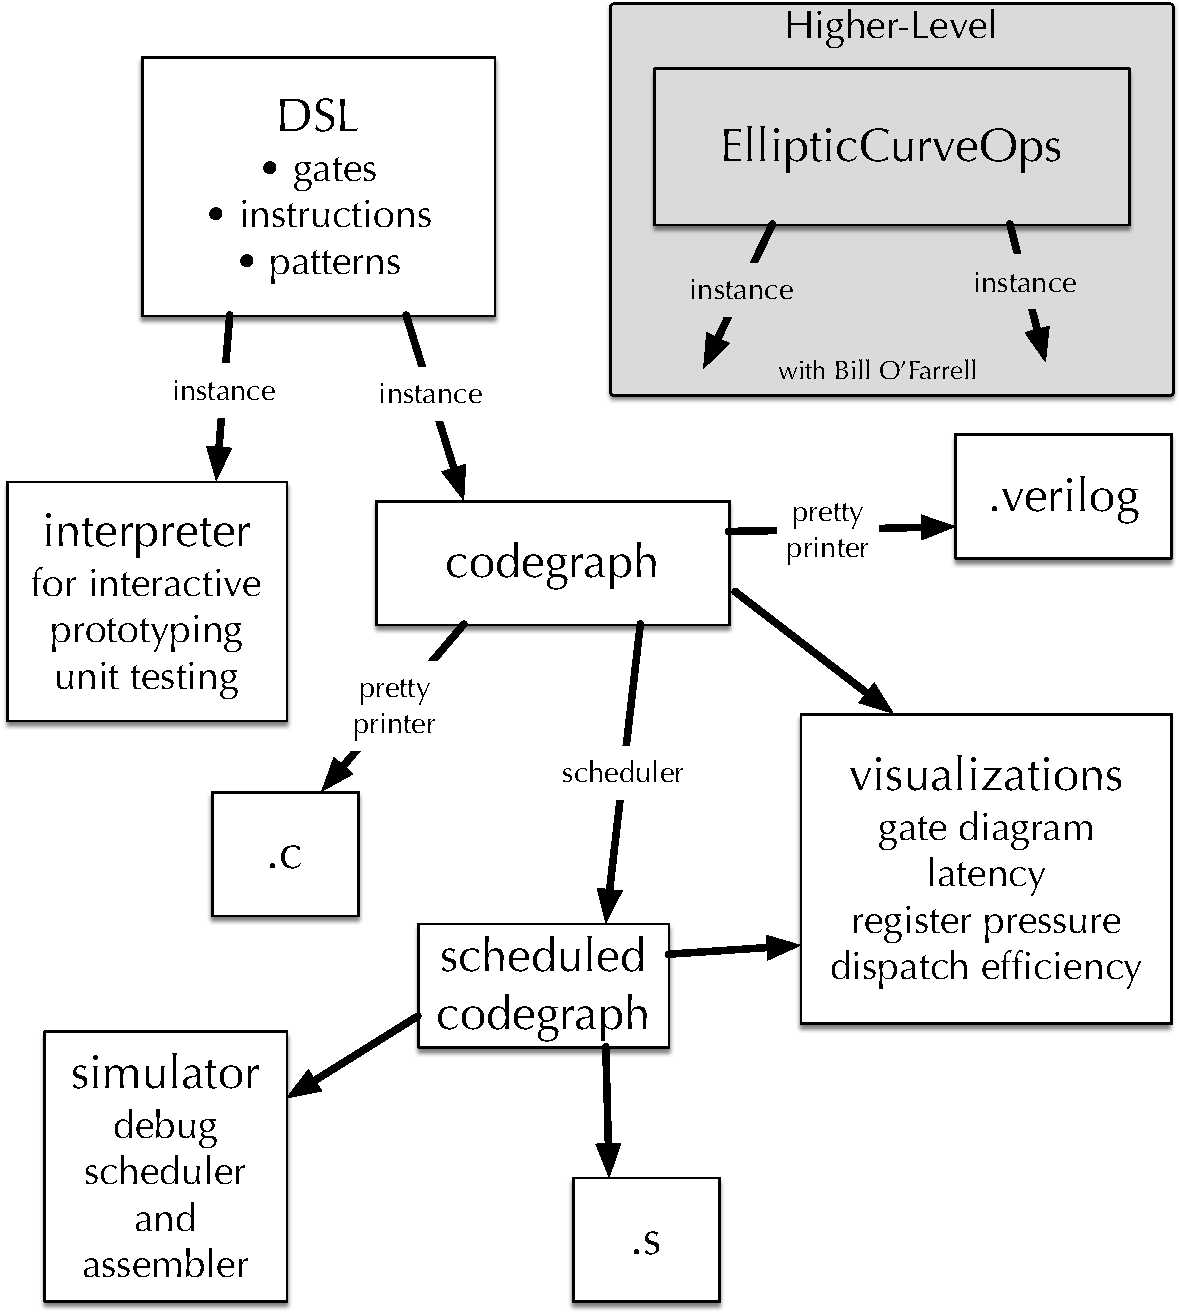
\includegraphics[width=0.6\textwidth]{figs/Coconut.pdf}
\end{figure}
\end{frame}

\begin{frame}{MDD - Coconut}
\begin{figure}
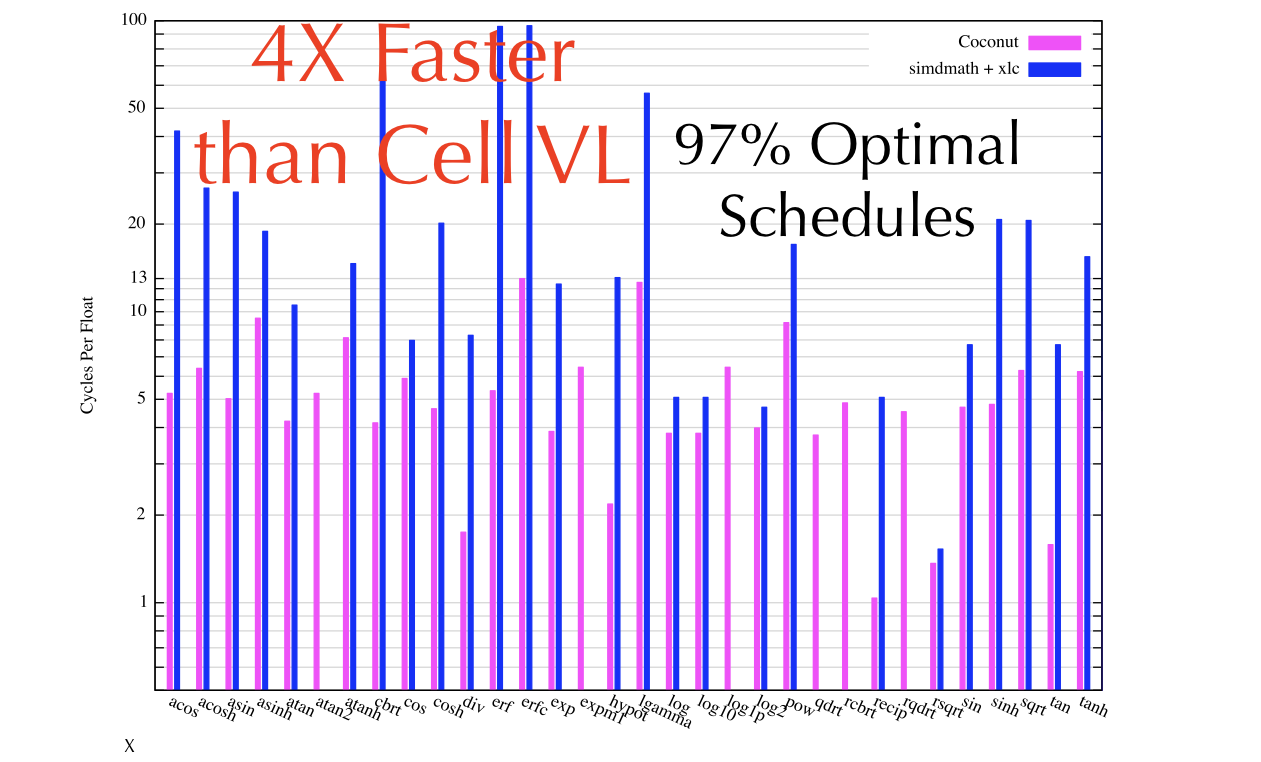
\includegraphics[width=0.9\textwidth]{figs/CoconutFaster.png}
\end{figure}
\end{frame}

\begin{frame}{MDD - Coconut}
\begin{itemize}
\item COde CONstruction User Tool
  \begin{itemize}
  \item used to generate MASS for all IBM platforms since Cell/B.E.
  \item but not used by users outside McMaster / OCA
  \item why?
    \begin{itemize}
    \item have to learn Haskell
    \item too many interfaces geared to abandoned research projects
    \end{itemize}
  \item fix = fix up the code
    \begin{itemize}
    \item open source!
    \item potential embarrassment will motivate clean up
    \end{itemize}
  \item open Coconut in pieces
  \end{itemize}
\end{itemize}
    \begin{tabular}{|l|l|l|}
    \hline
     today &  HashedExpression & calculus used for continuous optimization \\
    \hline
     later &  CodeGraph library & Intermediate Lanugage \\
    \hline
     later &  DSLs + interpreters &  front-ends \\
    \hline
     later &  scheduler + simulator & back-end \\
    \hline
    \end{tabular}
\end{frame}


\section{Optimization}
\label{sec:org49ebdff}
\begin{frame}[label={sec:orgd027c63}]{Optimization}
  \begin{itemize}
  \item maximize benefit
  \item minimize cost
  \item satisfy constraints
  \item make anything better!
  \item not just instruction scheduling
  \end{itemize}
\end{frame}

\begin{frame}{Optimization - MRI}
\begin{figure}
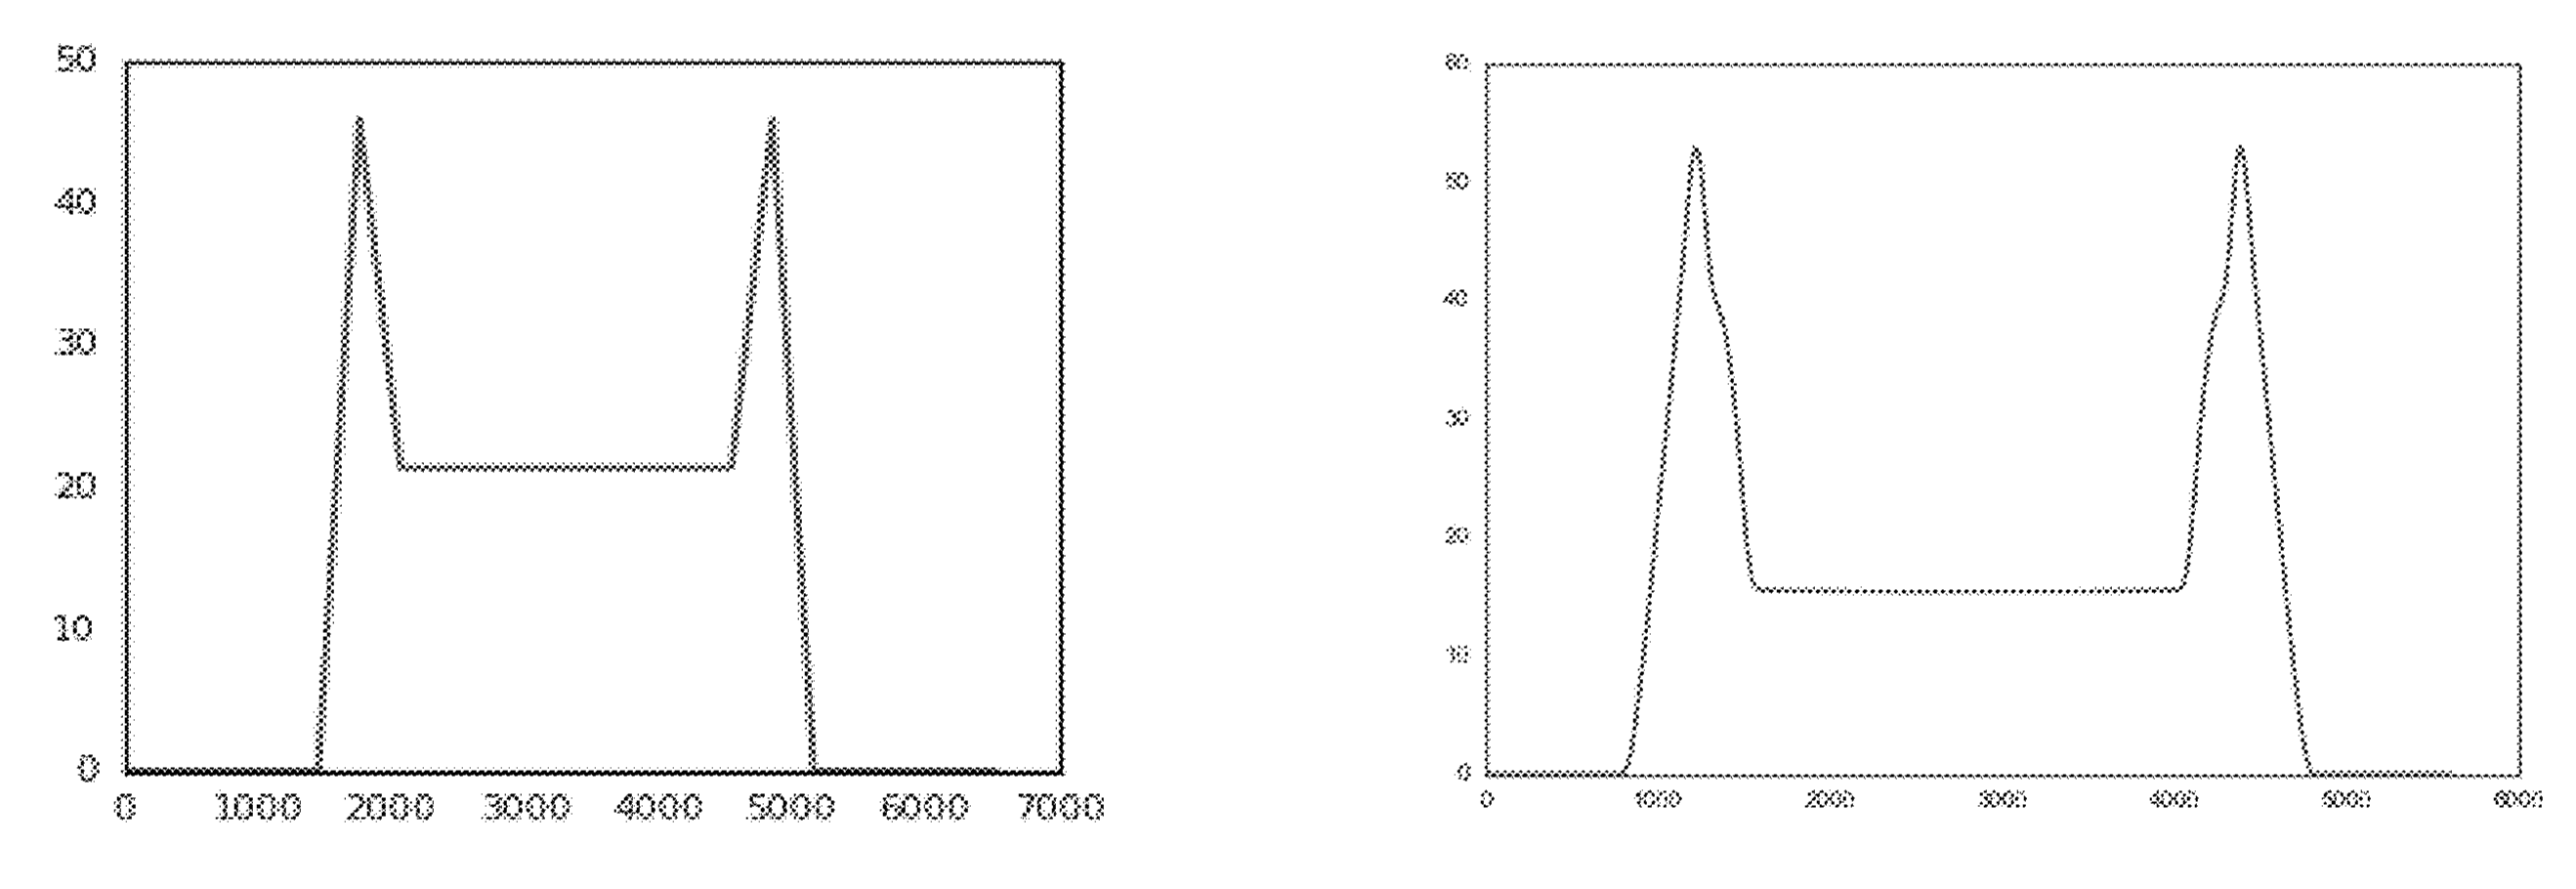
\includegraphics[width=0.9\textwidth]{figs/BeforeAfterMRI.png}
\end{figure}
  \begin{itemize}
  \item big and little magnets manipulate proton spins
  \item antenna picks up signal
  \item little magnets controlled by ``gradient waveforms''
  \item common designs (left) are not realizable
  \item reformulate as an optimization problem (producing right)
  \end{itemize}
\end{frame}

\begin{frame}{Optimization - MRI}
  \begin{itemize}
  \item key insight:  important waveforms are periodic
  \item Fourier Transform is discrete
  \item optimize over finite set of coefficients
  \end{itemize}
\begin{align}
 \operatorname{min}_{\{h_f:f\in F\}}\quad & \delta \\
   \text{subject to}\quad & \left| \mu - g(t) \right| \le \delta, \qquad \forall t \in S \\
   & \left| g(t) \right| \le g_{\text{peak}}, \qquad \forall t \\
   & \left| \partial g / \partial t (t) \right| \le g_{\text{slew}}, \qquad \forall t \\
   & \int_{ t \in S } g(t) = A \\
   \text{where}\quad & g(t) = \sum_{f\in F} h_f \sin(2\pi t f)
\end{align}
\end{frame}

\begin{frame}[label={sec:orgd027c63}]{Optimization - MRI}
  \begin{itemize}
  \item developed with AMPL/neos
  \item needed parametrized family for production
  \item reimplement in Python
  \item want one tool for development and deployment
  \end{itemize}
\begin{figure}
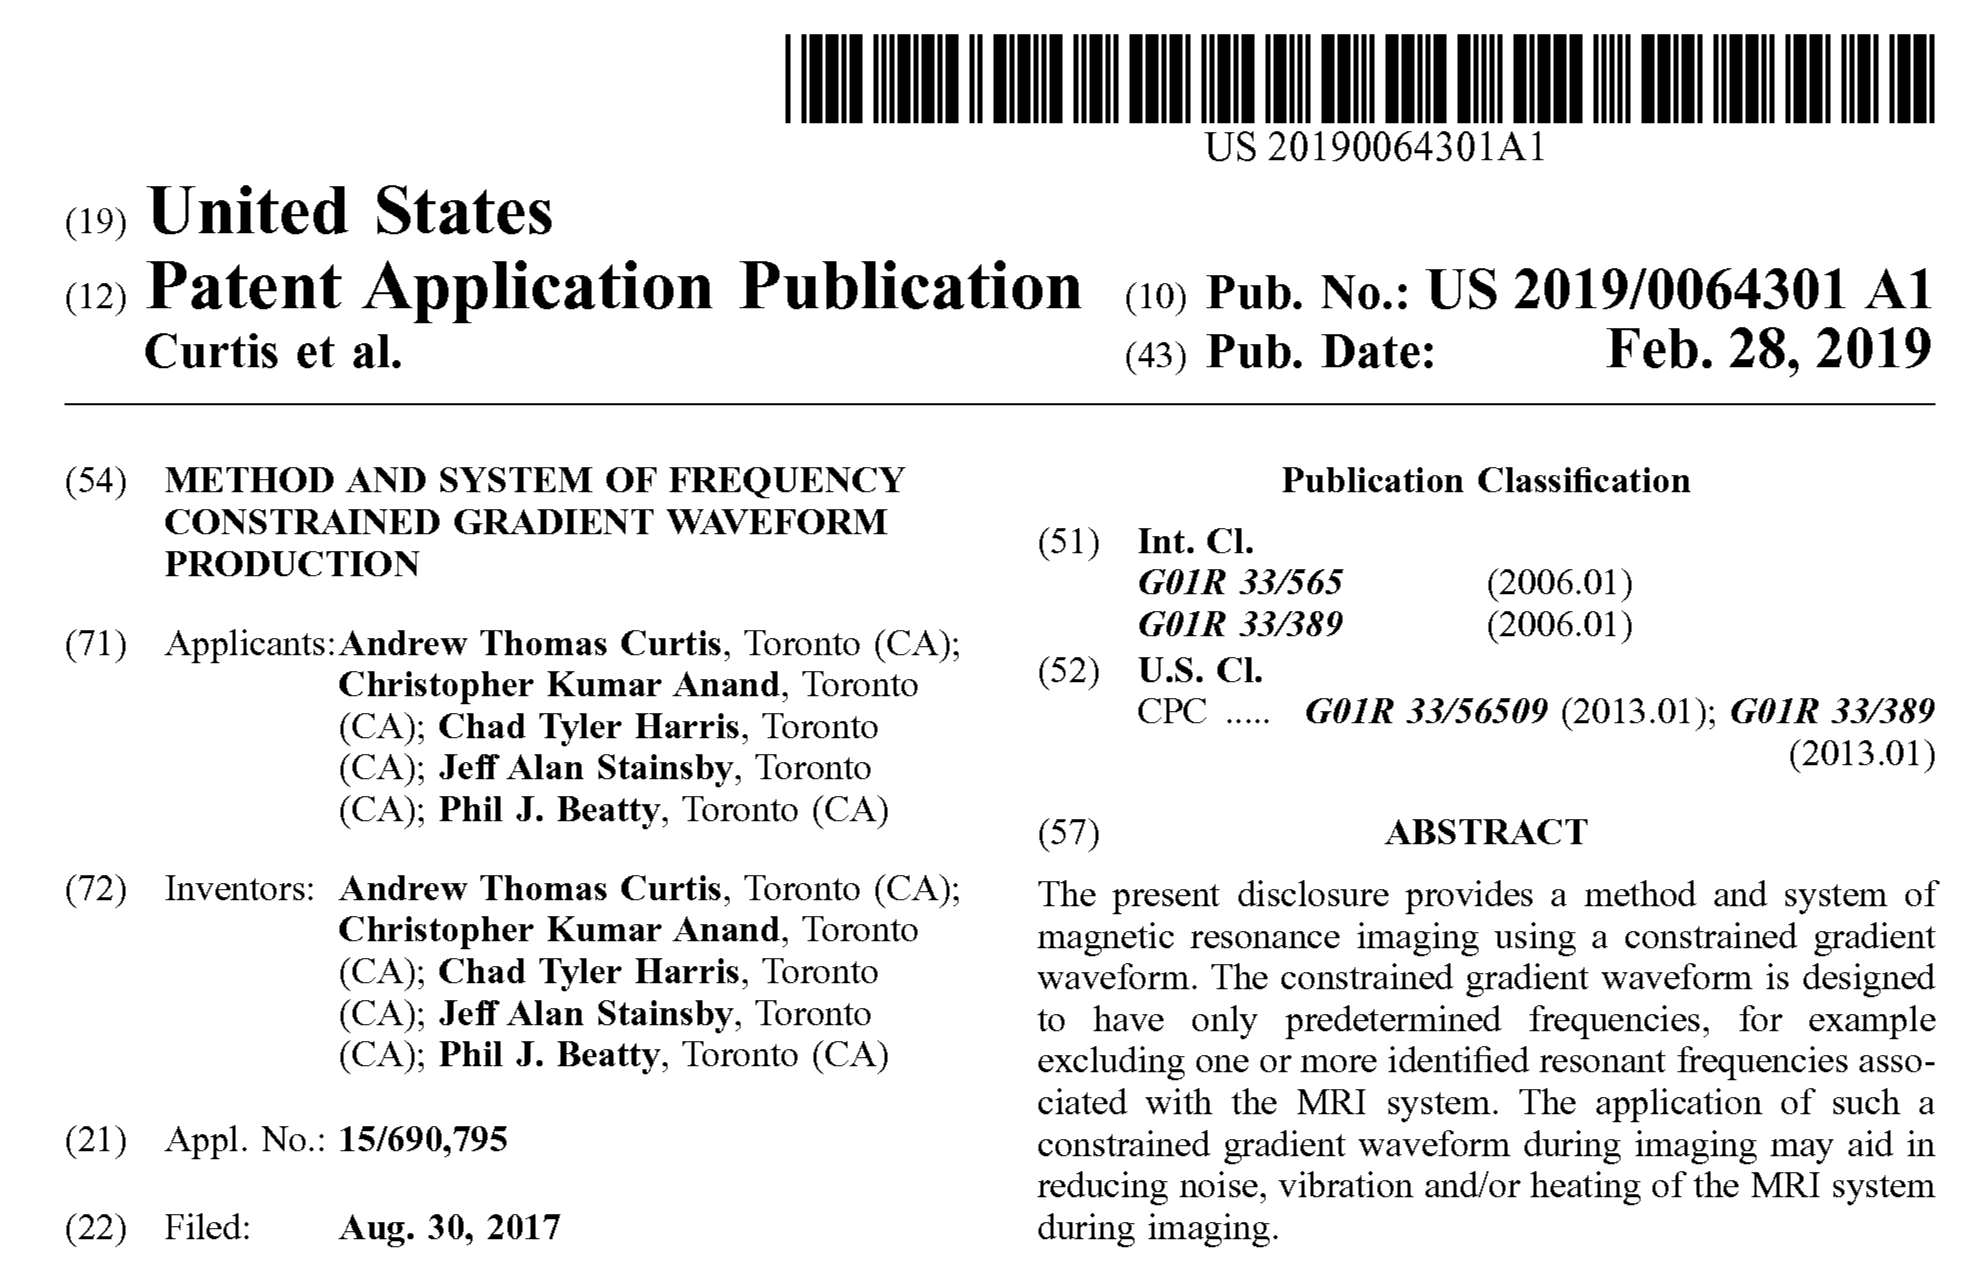
\includegraphics[width=0.5\textwidth]{figs/GradPatent.png}
\end{figure}
\end{frame}


\section{Example:  Parabola}
\label{sec:org6765f95}
\begin{frame}[label={sec:org0a594b7}]{Optimizing A Simple Parabola}
  \begin{columns}
    \begin{column}{0.5\textwidth}
      \begin{figure}
       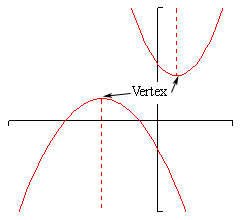
\includegraphics[scale=0.5]{figs/parabola.png}
       \caption{Example Parabola's: Solve for Vertex}
      \end{figure}
    \end{column}
    \begin{column}{0.4\textwidth}
      \begin{align}
        \min_x \quad & a x^2 + b x + c  \\
        \textsc{subject to } & x \leq n & \\
        & g(x) \leq m
      \end{align}
    \end{column}
  \end{columns}
\end{frame}

\begin{frame}[fragile]
  \frametitle{AMPL - MDD Solution for Optimization}
  \lstset{frame=tb,language=AMPL,aboveskip=3mm,belowskip=3mm,showstringspaces=false,columns=flexible,basicstyle={\ttfamily},numbers=none,numberstyle=\tiny\color{gray},keywordstyle=\bfseries,commentstyle=\textit,stringstyle=\color{mauve},breaklines=true,breakatwhitespace=true,tabsize=3}
  \begin{columns}
    \begin{column}{0.5\textwidth}
      \begin{figure}
\begin{lstlisting}
  param a;
  param b;
  param c;
  param n;
  param m;

  var x >= n;

  minimize Obj:
     a * x*x + b * x + c;

  subject to G:
     x * x <= m;
   \end{lstlisting}
   \caption{file: Quadratic.mod}
   \end{figure}
    \end{column}
    \begin{column}{0.5\textwidth}
      \begin{figure}
      \begin{lstlisting}
        data;

        param a := 1 ;
        param b := 0 ;
        param c := 5 ;
        param n := -10 ;
        param m := 0 ;
      \end{lstlisting}
      \caption{file: Quadratic.dat}
      \end{figure}
    \end{column}
   \end{columns}
\end{frame}

\begin{frame}
  \frametitle{Categories of Optimization Problems / Solvers}

  \begin{itemize}
  \item Many different categories of optimization
    \begin{itemize}
    \item Linear / Non-Linear
    \item Constrained / Un-Constrained
    \item Integer / Mixed Integer
    \item Semidefinite, stochastic, ...
    \end{itemize}
  \item Many, many different solvers to choose from
  \item No one to rule them all! (Optimization is not Lord of the Rings)
  \item NEOS Server: fantastic resource for running AMPL models on a variety of
    different solvers
    \url{https://neos-server.org/neos/solvers/index.html}
  \end{itemize}
\end{frame}

\begin{frame}
  \frametitle{Optimization Without MDD}

  \begin{itemize}
  \item Variety of solvers provide implemented in C / Java / Python
  \item however require you to supply auxiliary functions manually
  \item commonly required auxillary functions include:
    \begin{itemize}
    \item objective function
    \item gradient of the objective function
    \item hessian of the objective function
    \item constraint function(s)
    \item jacobian of the constraint function(s)
    \end{itemize}
  \end{itemize}
\end{frame}

\begin{frame}[fragile]
  \frametitle{Optimization Without MDD - C Example}

\begin{lstlisting}[style=CStyle]
void evaluate_partial_derivatives_and_objective() {
  ptr[OBJ] = ptr[A]*ptr[X]*ptr[X] + ptr[B]*ptr[X] + ptr[C];
  ptr[DERIVATIVE] = 2.0 *ptr[A]*ptr[X] + ptr[B];
}
void evaluate_objective() {
  ptr[OBJ] = ptr[A]*ptr[X]*ptr[X] + ptr[B]*ptr[X] + ptr[C];
}
void evaluate_partial_derivatives() {
  ptr[DERIVATIVE] = 2.0*ptr[A]*ptr[X] + ptr[B];
}
void evaluate_scalar_constraints() {
  ptr[CONSTRAINT] = pow(ptr[X],2);
}
void evaluate_scalar_constraints_jacobian() {
  ptr[CONSTRAINT_DERIVATIVE] = 2.0*ptr[X];
}
\end{lstlisting}
\end{frame}

\begin{frame}[fragile]
  \frametitle{Symphony - Middleground MDD}
  \begin{lstlisting}[style=CStyle]
    variables:
      x = 0

    constants:
      a = 1
      b = 0
      c = 5
      n = -10
      m = 0

    constraints:
      x <= n
      x^2 <= m

    minimize:
      a * x^2 + b * x + c   
  \end{lstlisting}
\end{frame}

\begin{frame}[fragile]
  \frametitle{Why Symphony?}
  \begin{itemize}
  \item no need to break out your Calculus 101 textbook
  \item generates just the auxiliary methods
  \item solver agnostic, plug into whatever c code you want
  \end{itemize}
\end{frame}

%%%%%%%%%%%%%%%%%%%%%%%%%%%%%%%%%%%%%%%%%%%%%%%%%%%%%%%%%%%%%%%%%%%%%%%%%%%%%%%%%%%%%
% User Manual (move to Part 2?)
%%%%%%%%%%%%%%%%%%%%%%%%%%%%%%%%%%%%%%%%%%%%%%%%%%%%%%%%%%%%%%%%%%%%%%%%%%%%%%%%%%%%%

\section{Symphony: User Manual}

\begin{frame}
  \frametitle{Vectors and dimension}
  \begin{itemize}
    \item In Symphony, everything is vector.
    \item Vectors
      \begin{itemize}
    \item Dimension (Shape): can be scalar, 1D, 2D, 3D, ...
      \begin{itemize}
      \item Scalar is just a single number 
      \item 1D(n) variable is an array of n number, useful for problems in signal processing, sound processing, ..
      \item 2D(m x n) variable is a 2D array of m x n numbers, useful for problems in image processing, ...
      \item 3D(m x n x p) variable is a 3D array of m x n x p numbers, useful for
        problems in topology, image processing with voxels, ...
      \end{itemize}
    \item Numtype: can be real (R) or complex (C)
      \end{itemize}
    \item We can manipulate vectors like adding, multiplying, doing inner product, ... to form new vectors (expressions).
  \end{itemize}
\end{frame}

\begin{frame}[fragile]
  \frametitle{Forming An Expression}

  \begin{itemize}
    \item $(+),(-),(*),(/)$ Add/Subtract/Multiply/Divide (point-wise) two vectors having same shape and same numtype
    \item $(*.)$ Scale a vector with a scalar (if they form a vector space in Mathematics, i.e, real number can scale anything, 
    but complex can only scale complex)
    \item $(\textsc{<.>})$ Inner product (dot product) of two vectors 
    \item (\^{}) Power a vector with an integer
    \item Piecewise:
    \begin{lstlisting}[style=Haskell]
    case x:
      x <= 0    -> -x
      otherwise -> x
    \end{lstlisting} 
    \item sumElements, norm2square, normHuber
  \end{itemize}
\end{frame}

\begin{frame}[fragile]
  \frametitle{Structure}
  A valid symphony problem consists of:
  \begin{itemize}
  \item Variables 
  \item Objective function 
  \item Constants (optional)
  \item Constraints (optional)
  \end{itemize}
\end{frame}

\begin{frame}[fragile]
  \frametitle{Variable Declaration}

  \begin{itemize}
  \item Variables are declared in a {\color{red} variable} block
  \item For example:
  \begin{lstlisting}[style=Haskell]
  variables:
    x[100][100] = 10
    y[20][20][20]
    a, b = 2, c
  \end{lstlisting}
  \item Assignment denotes an initial value
  \item Unassigned variables will be randomly initialized with a number between (0,1)
  \end{itemize}
\end{frame}

\begin{frame}[fragile]
  \frametitle{Objective Function}

  \begin{itemize}
  \item Declared in a {\color{red} minimize} block
  \item For example:
  \begin{lstlisting}[style=Haskell]
  minimize:
    (x - y)^2
  \end{lstlisting}
  \item Must evaluate to a scalar.
  \end{itemize}
\end{frame}

\section{Parts II and III}

\begin{frame}{Parts II and III}
  \begin{itemize}
  \item More Optimization: 
  \begin{itemize}
  \item example: Integrating Blood Flow from PCA-MRI
  \item example: MRI Image Reconstruction with Mask
  \item example: Parallel MRI
  \item example: Logistics
  \item Hashed Expression (Symphony's Backend)
  \end{itemize}
  \item PAL:  Petri App Land
  \begin{itemize}
  \item State Diagrams can model user interaction (grade 5+)
  \item PALDraw:  graphical modelling tool for State Diagrams
  \item make a working app
  \item Petri Nets can model multi-user interaction in web apps
  \item PALDraw:  graphical modelling tool for Petri App Land
  \end{itemize}
  \end{itemize}
\end{frame}

\end{document}